\chapter{Обзор системы VLC}

\section{Li-Fi и VLC}

\Abbrev{IM}{intensity modulation}
\Abbrev{DD}{direct detection}
\Abbrev{IEEE (Institute of Electrical and Electronics Engineers)}{институт электроники и инжинеров электроники}

В VLC данные передаются при помощи модуляции интенсивности излучения источника (светодиода) \--- IM. Приёмником в такой системе может выступать фотодетектор, который использует принцип прямого детектирования (DD). VLC был придуман для связи <<от точки к точке>>, то есть как замена кабелям~\cite{Haas16}. Работа VLC описывается стандартом IEEE 802.15.7-2018~\cite{IEEE2018}.

С другой стороны, Li-Fi описывает полную беспроводную сеть с возможностью двусторонней коммуникации <<от точки к многим точкам>> и  <<от многих точек к точке>>. Помимо этого, Li-Fi включает в себя возможность использования многих точек доступа с быстрым переключением между ними, что позволяет обеспечить мобильность пользователей. То есть стандарт Li-Fi включает в себя стандарт VLC, что показано на схеме \ref{fig:vlcvslifi}.

\begin{figure}[!ht]
    \centering
    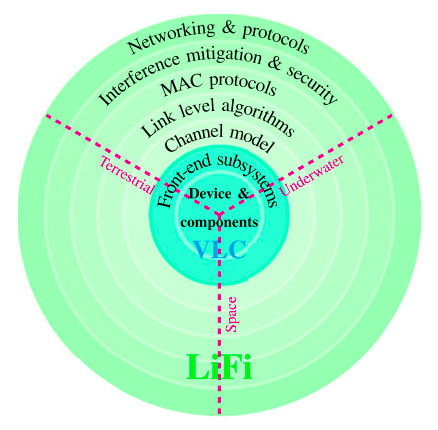
\includegraphics[width=.6\textwidth]{inc/img/vlcvslifi.png}
    \caption{Принципиальная схема Li-Fi и VLC~\cite{Haas16}}
    \label{fig:vlcvslifi}
\end{figure}

Как и было описано во введении, Li-Fi имеет ряд преимуществ по сравнению с Wi-Fi: он позволяет обеспечить безопасность передачи данных, отсутствие интерференции с ЭМ-приборами, разгрузка РЧ-спектра.

\section{Li-Fi передатчик}

Зачастую в системах передачи информации с помощью видимого света в качестве передатчика выбирается светодиодный светильник (LED luminaire)~\cite{LeMinh2008,Komine2006,Komine2004}. Он представляет из себя полноценное осветительное устройство, состоящее из LED источник излучения, балласта, корпуса и других компонентов. LED источник может состоять из одного или нескольких светодиодов, которые управляются с помощью управляющей микросхемы \--- контроллера, который контролирует ток, питающий светодиод и меняющий его яркость. Когда светодиодный светильник используется для коммуникации, контроллер модернизируется для передачи данных с помощью модуляции излучения. Примером простейшей модуляции является On-Off Keying, то есть <<нули>> и <<единицы>> передаются как два разных уровня интенсивности света.

Ключевым требованием к конструкции системы Li-Fi является то, что освещение, которое является основной целью светодиодных светильников, не должно нарушаться из-за использования связи. Таким образом, на работу Li-Fi системы влияет конструкция светодиодного светильника. Белый свет является самым используемым для освещения в помещениях и на улице. Это связано с тем, что цвет предметов под белым светом наиболее сильно похож на цвет предметов под естественным светом. Белый свет у LED светильников достигается двумя разными способами: 

\begin{enumerate}
    \item Синий LED с фосфором \--- этот источник генерирует белый свет с использованием синего LED, который покрыт жёлтым фосфором. Когда синий свет проходит через жёлтое покрытие, эта комбинация создаёт белый свет. При изменении толщины покрытия можно получать белый свет различной цветовой температуры.
    \item Комбинация RGB светодиодов \--- белый свет может быть получен при смешении красного, зелёного и синего света. Для этого, соответственно, необходимо три светодиода, что повышает стоимость светильника, по сравнению с синим фосфорным LED. 
\end{enumerate}

В осветительных системах чаще всего используется первый тип светодиодов из-за их дешевизны, однако в коммуникационных системах фосфорное покрытие значительно ограничивает скорость, с которой светодиод можно переключать, до нескольких МГц~\cite{Khalid2012}. С другой стороны, использование нескольких цветных светодиодов позволяет использовать Color Shift Keying модуляцию при помощи трёх длин волн, что позволяет получить высокую скорость передачи данных и низкую стоимость LED~\cite{Bian2019}.

\section{Li-Fi приёмник}

В качестве приёмников в Li-Fi системах чаще всего используются

\begin{enumerate}
    \item фотодетекторы \--- фотодиоды,
    \item датчики изображения \--- камеры.
\end{enumerate}

Фотодетектор \--- полупроводниковое устройство, которое генерирует ток при падении на него света. Современные коммерческие фотодетекторы могут детектировать с частотой до десятков МГц. 

\Abbrev{FPS (frames per second)}{кадры в секунду}
\Abbrev{IoT (internet of thing)}{интернет вещей}

Помимо него, возможно и использование камеры, так как они уже встроены в большинство потребительской техники (смартфоны, ноутбуки), что позволяет сделать эти устройства приёмниками в Li-Fi системе. Помимо этого, открывается возможность использования Li-Fi для интернета вещей (IoT)~\cite{Duquel2018}. По сути, камера является матрицей фотодетекторов на плате. Существенным недостатком является то, что так как камеры приспособлены для получения изображений высокого разрешения, используется большое количество фотодетекторов, что значительно снижает количество кадров в секунду (FPS) \--- скорость обработки излучения. Например, камеры современного смартфона позволяют записывать видео с 60 FPS, что означает, что использование камеры значительно ограничивает скорость получения информации. 

Важно отметить, что несмотря на то, что использование камеры позволяет превратить любое мобильное устройство в приёмник, пропускная способность остаётся очень ограничена (порядка килобит в секунду). В то же время отдельные фотодетекторы позволяют принимать информацию с высокой пропускной способностью (сотни мегабит в секунду).

\section{Методы модулирования излучения}

% http://www.phpathak.com/files/vlc-comsoccst.pdf p 10

Самое важное отличие системы связи по видимому свету от РЧ-связи заключается в том, что в VLC информация не может быть закодирована в амплитуде и фазе света~\cite{Tsonev2013}. Это означает, что техники модуляции, использующие модулирование фазы и амплитуды не могут быть применены в VLC, и информация должна быть закодирована в интенсивности света \--- модуляция интенсивности (IM). При создании Li-Fi системы необходимо учитывать параметры освещения, некоторые из которых могут повлиять на человека. Пример таких параметров: 
% Существуют различные техники модуляции интенсивности, некоторые из них будут рассмотрены ниже.

\begin{enumerate}
    \item затемнение\footnote{dimming}. В~\cite{Zukauskas2002} было показано, что для разных действий необходимы разные уровни яркости освещения. Например, освещение в интервале $30-100$ лк обычно является достаточным для освещения общественных мест. С другой стороны, для освещения офисов и домов необходима освещённость порядка $300-1000$ лк. Благодаря развитию технологии светодиодных драйверов, становится возможно затемнять светодиоды до любого необходимого уровня в зависимости от применения и требований по сохранению энергии;
    \item смягчение мерцания\footnote{flicker mitigation}. Для системы коммуникации по видимому свету необходимо, чтобы человек не замечал мерцание яркости света. В~\cite{Berman1991} было показано, что мерцание может вызывать серьезные физиологические последствия у людей. Поэтому, необходимо модулировать свет с более высокой частотой, чем частота, которую может воспринимать человеческий глаз. В стандарте IEEE 802.15.7~\cite{IEEE2018} предложено использовать модуляцию интенсивности с частотой выше 200 Гц для избежания вреда для здоровья. 
\end{enumerate}

Рассмотрим четыре типа модуляции, которые применяются в VLC: 

\Abbrev{ИМ}{импульсная модуляция}
\Abbrev{CSM}{color shift modulation}

\begin{enumerate}
    \item On-Off Keying (OOK);
    \item импульсная модуляция (ИМ);
    \item мультиплексирование с ортогональным частотным разделением каналов;
    \item color shift modulation (CSM);
\end{enumerate}

\subsection{On-Off Keying}

\Abbrev{NRZ}{non-return-to-zero [on-off-keying]}

В OOK биты данных 1 и 0 передаются включением и выключением светодиода соответственно. В выключенном состоянии светодиод не выключен до конца, но интенсивность его излучения уменьшена. К преимуществам OOK относят простоту реализации. Схожая модуляция используется в волоконных коммуникациях. Большинство ранних работ с использованием OOK в VLC использовали белый светодиод. Если используется синий светодиод с фосфором, то его пропускная способность сильно ограничена (в связи с временем релаксации \--- несколько МГц~\cite{Grubor2007}). Было предложено~\cite{Park2007} использовать <<не возвращающийся к нулю>>\footnote{non-return-to-zero (NRZ)} OOK с синим светодиодом, то можно достичь пропускной способности порядка десятков Мб/с. Помимо этого, можно использовать~\cite{Grubor2007} синий фильтр, чтобы из сигнала медленно реагирующий жёлтый фосфор, в результате чего повысив скорость передачи данных до 40 Мб/c. Аналогично в~\cite{Minh2008,Vucic2009} было предложено комбинирование синего фильтра и аналогового выравнивания на приёмнике для достижения скорости передачи данных 100 и 125 Мб/с соответственно. В~\cite{Vucic2010} было показано, что производительность можно увеличить при помощи лавинных фотодиодов (а не p-i-n фотодиод) в качестве приёмника. Достижимая скорость передачи данных с лавинным фотодиодом и NRZ-OOK составила около 230 Мб/с~\cite{Vucic2010}. В~\cite{Fujimoto2013} использовался RGB светодиод (который лишен основного недостатка фосфорных светодиодов \--- ограничения частоты модуляции из-за времени релаксации). Однако в этой работе модуляция происходила только по одному цветовому каналу \--- красному, в то время как остальные были использованы для создания постоянного белого освещения. Полученная система достигла скорости передачи данных 477 Мб/с с простой NRZ-OOK модуляцией и p-i-n фотодиодным приёмником. 

\subsection{Методы импульсной модуляции}

\Abbrev{PWM (pulse width modulation)}{модуляция длительности импульса}
\Abbrev{PPM (pulse position modulation)}{фазово-амплитудная модуляция}

Несмотря на то, что OOK имеет ряд преимуществ (простота и лёгкость реализации), оно имеет значительное ограничение \--- низкая скорость передачи данных. Поэтому были разработаны альтернативные методы модуляции, которые основаны на длительности (PWM) и положении импульса (PPM). 


\subsubsection{Модуляция длительности импульса}

PWM является эффективным способом модуляции при помощи затемнения. При PWM длительность импульсов выбирается исходя из желаемого уровня затемнения, в то время как сами импульсы несут модулированный сигнал. Этот сигнал передается в импульсе, во время которого светодиод работает на полной мощности. В~\cite{Sugiyama2007} было показано, что затемнение от $0\%$ до $100\%$ может быть получено с высокой частотой PWM. Одним из преимуществ PWM является возможность достижения затемнения без изменения интенсивности импульсов, что не приводит к изменению цвета (что может происходить в OOK). К ограничениям PWM можно отнести ограниченную скорость передачи данных (4.8 Кб/с в~\cite{Sugiyama2007}). Для 

% To overcome this limitation, [44] proposed
% to combine PWM with Discrete Multitone (DMT) for joint
% dimming control and communication. The approach decouples
% the dimming based on PWM and communication based on
% DMT on the transmitter side. As shown in Fig. 13, the bitstream
% is divided and mapped to symbols using Quadrature Amplitude
% Modulation (QAM). These QAM symbols are transmitted on
% different DMT subcarriers that are spaced by 1/T in frequency
% where T is the duration of one symbol. The DMT signal x(t) is
% combined with PWM square wave signal p(t) where the duty
% cycle is dependent on desired level of dimming. The resultant
% signal y(t) = x(t)p(t) is shown in Fig. 13. It was also shown
% that dimming constraint limits the achievable throughput due to
% high Bit Error Rate (BER). Authors in [46] also used QAM on
% DMT subcarriers to achieve a link rate of 513 Mbps, however,
% it does not address the issue of LED dimming.